\chapter{STUDY III - INNER SIDE DIAGNOSIS IMPROVEMENT }\label{chp:Inner Side Diagnosis Improvement}

This chapter focuses on arch high index calculation improvements with the data provided in Chapter \ref{chp:Back Side Diagnosis}. Accordingly, Section \ref{sec:StudyIIIAnalysisAndDesign} will cover analysis and design decisions. Then, in Section \ref{sec:StudyIIIImplementation}, delves into the specifics of implementation. Finally, the initial test findings and evaluation phase will be discussed in Section \ref{sec:StudyIIITestAndEvaluation}.

\section{ANALYSIS AND DESIGN}\label{sec:StudyIIIAnalysisAndDesign}

Preliminary detection of potential pes planus and pes cavus patients will be provided based on the inner side photographs of the foot. This system will be based on the initial implementation of the arch height index calculation discussed in Chapter \ref{chp:Foot Detection & Primary Diagnosis}. However, this chapter profoundly focuses on improving the batch process on pre-diagnosis.

Tree major fallbacks of the initial design were discovered in the test end evaluation of the process. All the fallbacks and potential solutions will be discussed in the following paragraphs.  

The first fallback is the differences between the line of the sole and the symmetry of the sole function. These differences should be reduced, and the foot function's sole should be more accurate.

The second fallback is that the bottom of the images contains a lot of noise in edge detection. By eliminating these noises, the accuracy of the sole foot function should be increased. The greedy approach could be used to improve accuracy with a relatively less computational resource.

The third fallback is that there is no error detection mechanism to reduce the error. Therefore, the sole function should not only be used for point detection but also for detecting the slope of the foot. As a result, this feature extraction should be used for detecting anomalies so that the results can be corrected.

\section{IMPLEMENTATION}\label{sec:StudyIIIImplementation}

Implementation details of the changes in the batch process will be discussed in this section. Each change will be separately discussed for a detailed explanation.

\begin{figure}[htbp]
\centering
\fbox{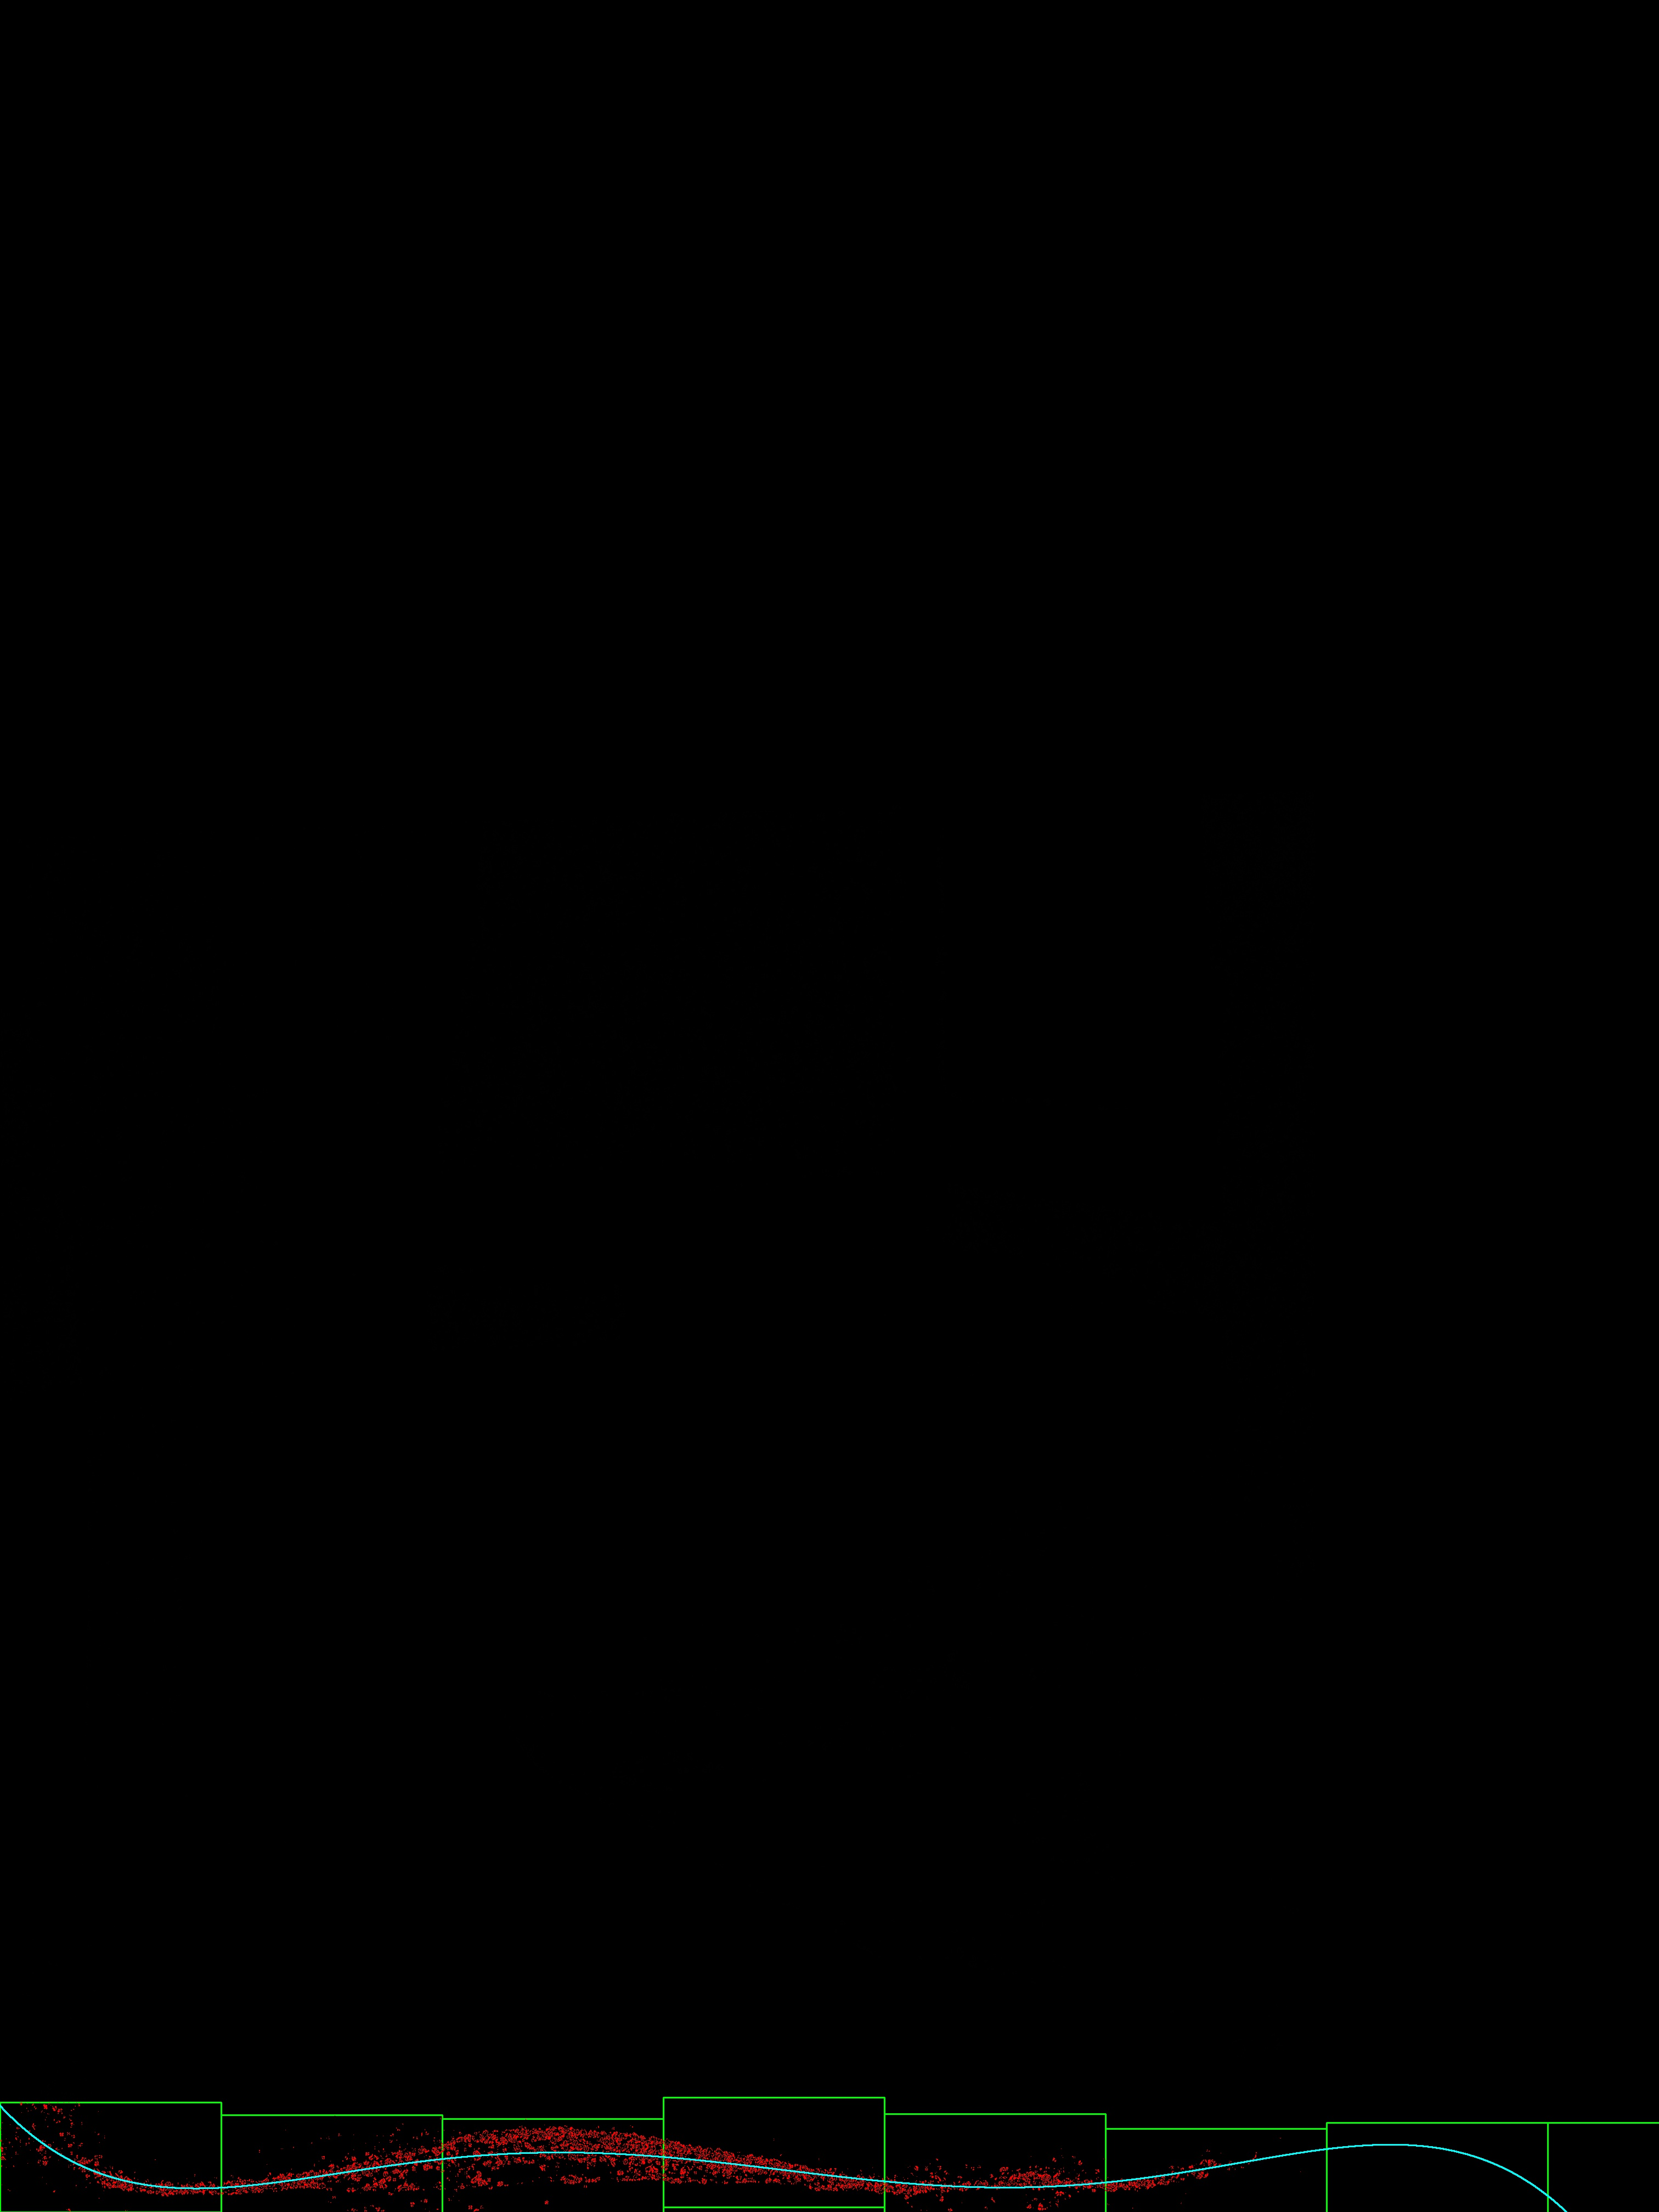
\includegraphics[width=.60\columnwidth]{KaanEksenMSc/figures/StudyIIIPredefinedWindows.jpeg}}
\caption{Accuracy improvement with polynomial regression window in study III}
\label{fig:StudyIIIPredefinedWindows}
\end{figure}

The first fallback is the accuracy of the sole function. The sole function generation was designed to reduce the sudden slope changes to the function because there might be an error in edge detection. Increasing the predefined windows, where polynomial regression is applied, will improve the function's response to changes (see Figure \ref{fig:StudyIIIPredefinedWindows}).

\begin{figure}[htbp]
\centering
\fbox{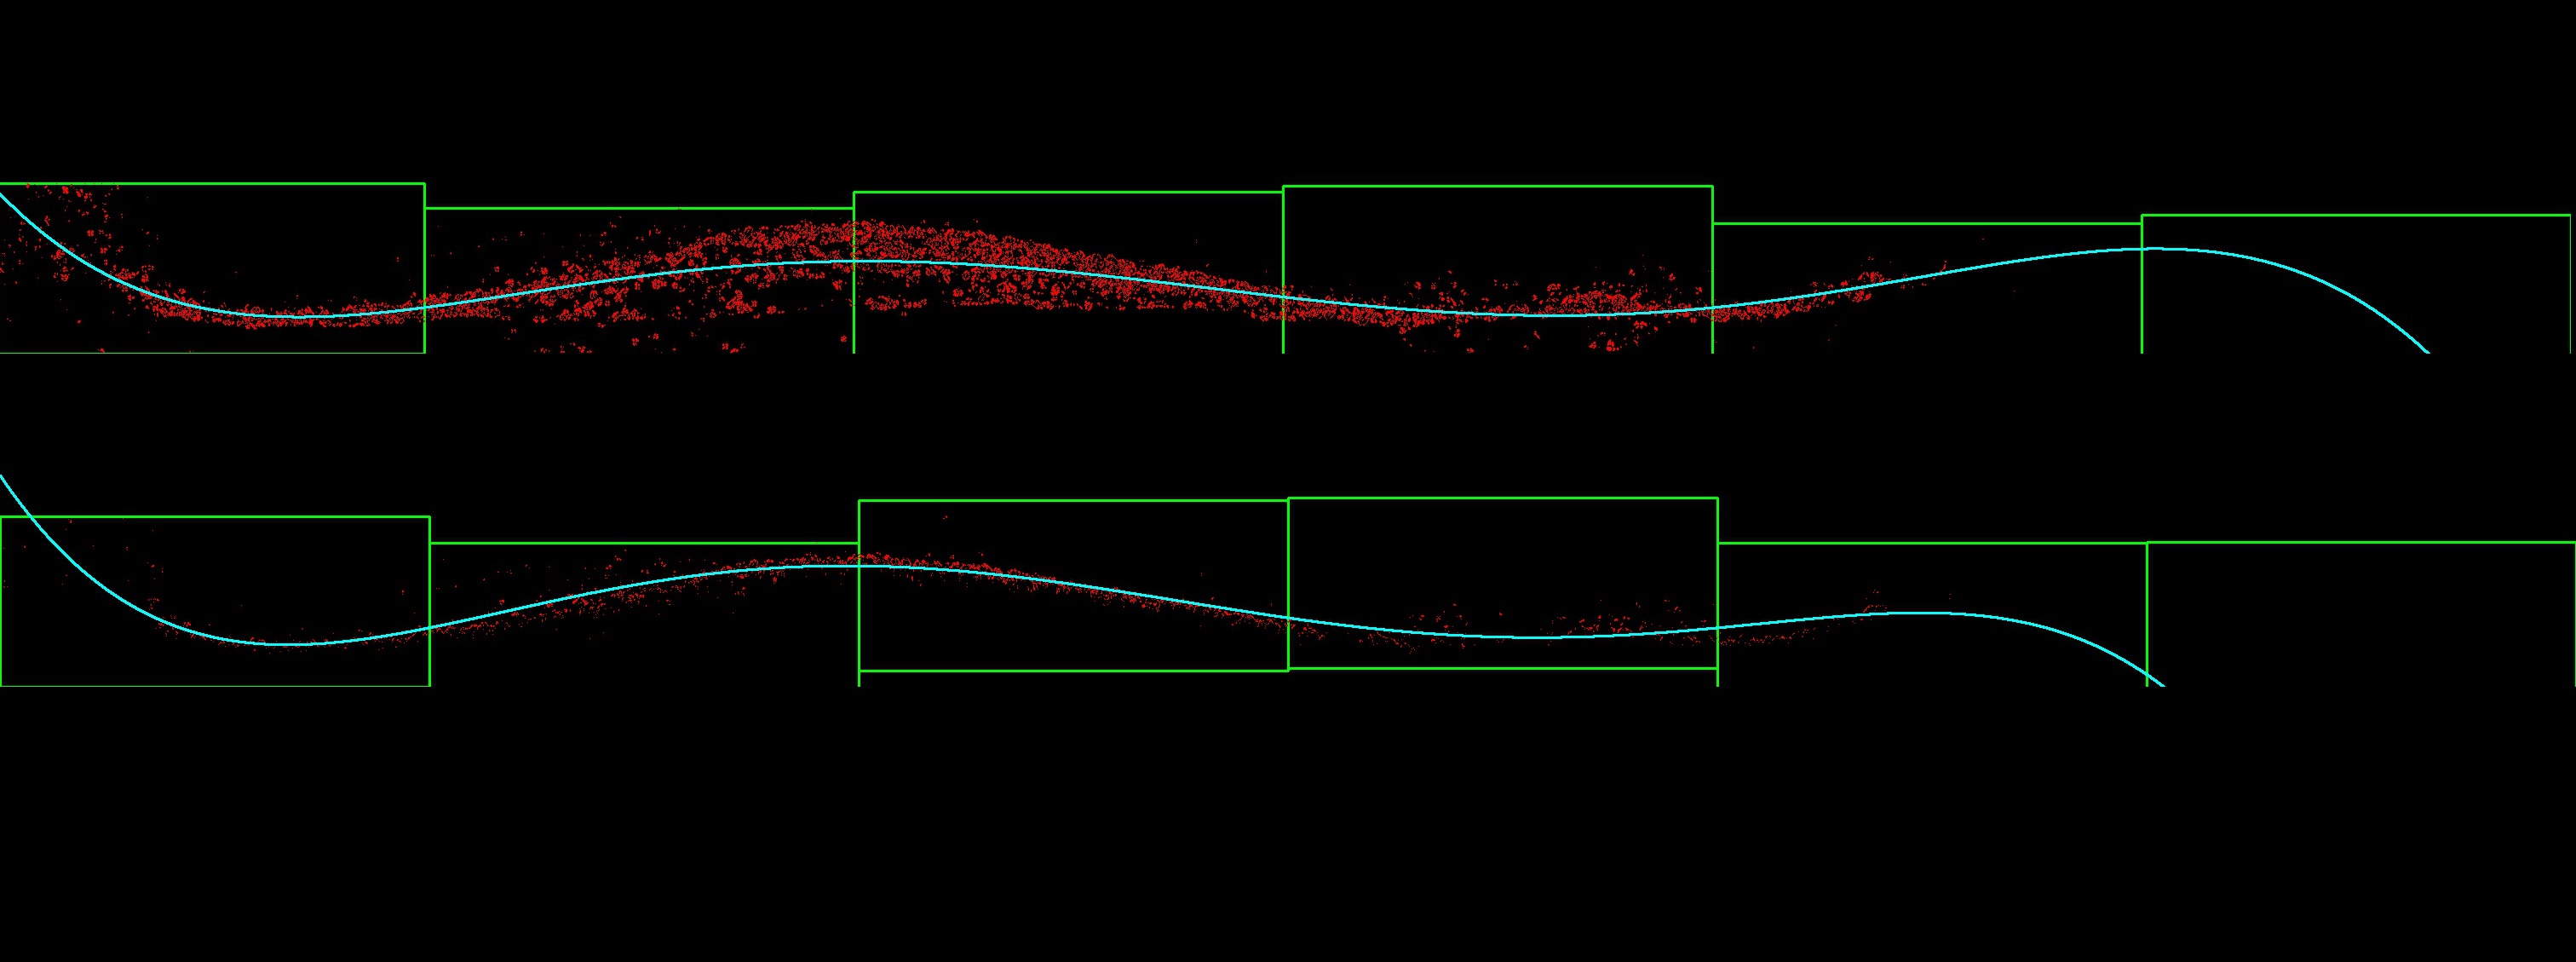
\includegraphics[width=.80\columnwidth]{KaanEksenMSc/figures/StudyIIINoiseReduce.jpg}}
\caption{Greedy noise reduce improvement in study III}
\label{fig:StudyIIINoiseReduce}
\end{figure}

The second fallback is that the edge images contain noise. Since the bottom of the images is changing based on the floor decoration,  removing the remaining edges on the floor will significantly improve the sole function accuracy. Since the foot has not contained edges in the bottom, actively removing the remaining edge 80 percent of points in the bottom should boost the accuracy (see Figure \ref{fig:StudyIIINoiseReduce}).

\begin{figure}[htbp]
\centering
\fbox{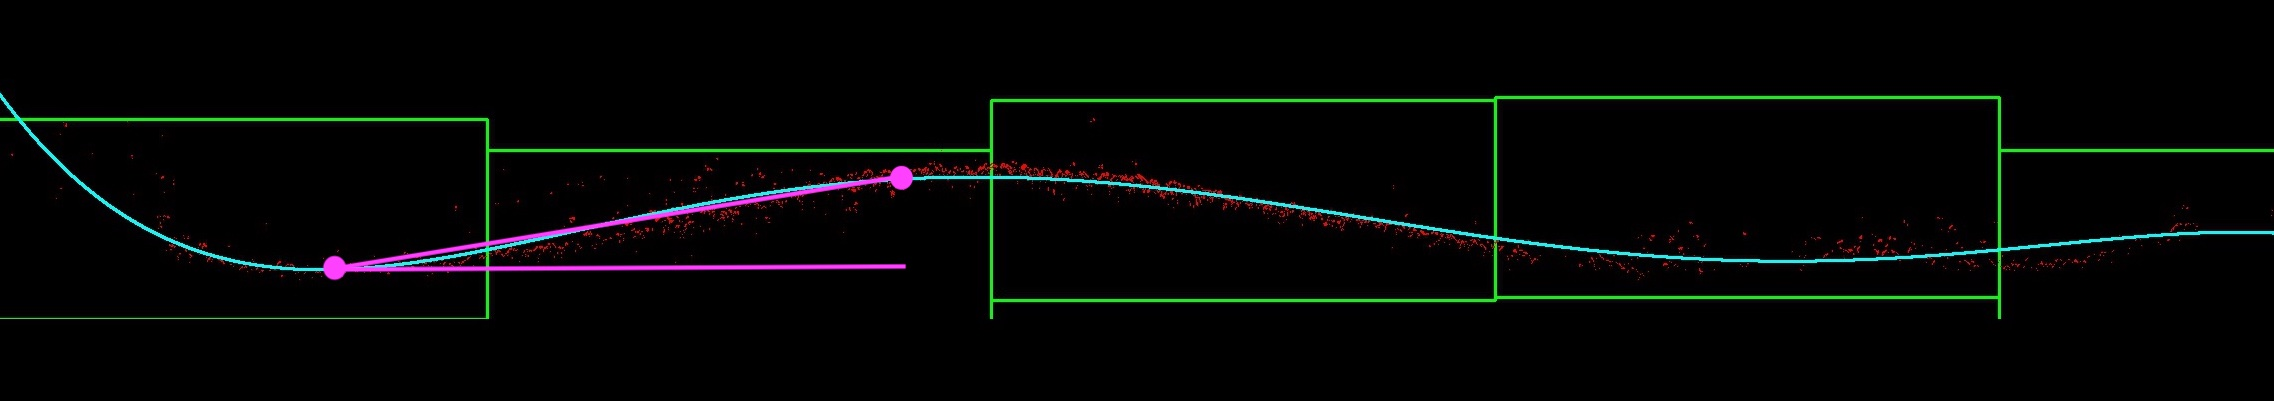
\includegraphics[width=.80\columnwidth]{KaanEksenMSc/figures/StudyIIISlopeCalculation.jpg}}
\caption{Slope calculation for error detection mechanism  in study III}
\label{fig:StudyIIISlopeCalculation}
\end{figure}

The last fallback is the absence of an error detection mechanism. With improved sole function, this can be achieved by calculating the function's slope in certain positions. The fact that the slope is higher than a specific rate is an indicator of pes cavus. Likewise, the same assumption can be made for the lack of slope. This error can be detected by taking two points in the foot; as the heel's peak and the foot space in the center (see Figure \ref{fig:StudyIIISlopeCalculation}).

\section{TEST AND EVALUATION}\label{sec:StudyIIITestAndEvaluation}

This section will provide the test end evaluation process of the prototype system described in detail in previous sections. In addition, thee were no data collection part. The third study uses the same data discussed in Section \ref{sec:StudyIITestAndEvaluation}. Therefore, the data collection and data details will be skipped.

\begin{figure}[htbp]
\centering
\fbox{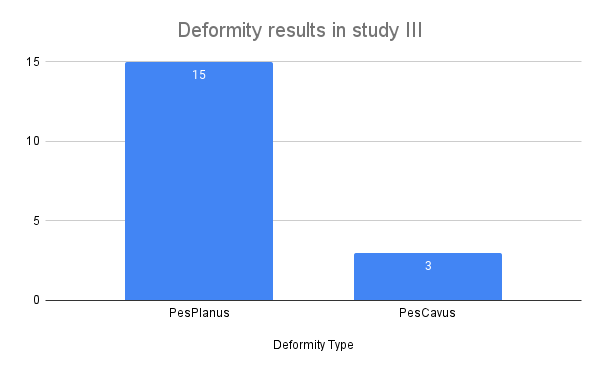
\includegraphics[width=.60\columnwidth]{KaanEksenMSc/figures/StudyIIIFootDeformityAutomatedProcessResults.png}}
\caption{Foot deformity distribution in automated process results in study III}
\label{fig:StudyIIIFootDeformityAutomatedProcessResults}
\end{figure} 

Initial results showed that the findings of the healthcare officials and the system were 83,3 percent matched (see Figure \ref{fig:StudyIIIFootDeformityAutomatedProcessResults}). There were one pes planus two pes cavus mismatch detection recorded. Improved inner side test results with slope calculation are promising (see Figure \ref{fig:StudyIIISlopeResults}). However, the population was not diverse. Therefore the system should be tested on a larger population to get more accurate results.

\begin{figure}[htbp]
\centering
\fbox{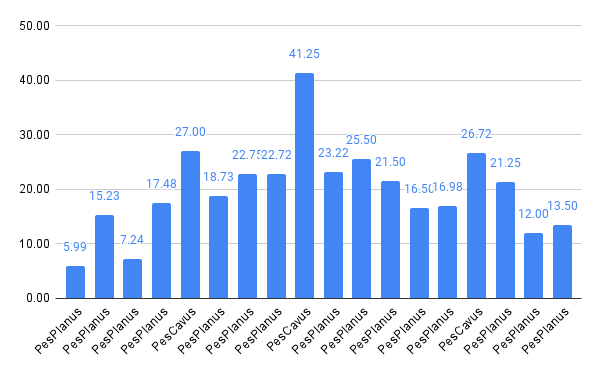
\includegraphics[width=.60\columnwidth]{KaanEksenMSc/figures/StudyIIISlopeResults.png}}
\caption{Foot deformity and calculated slope in automated process results in study III}
\label{fig:StudyIIISlopeResults}
\end{figure} 
